% Graphic for TeX using PGF
% Title: /comptes/E124582Q/L3/BDD/proj/wookie-hebdo/rapport/src/figures/tables_schema.dia
% Creator: Dia v0.97.2
% CreationDate: Fri Mar 20 13:48:47 2015
% For: E124582Q
% \usepackage{tikz}
% The following commands are not supported in PSTricks at present
% We define them conditionally, so when they are implemented,
% this pgf file will use them.
\ifx\du\undefined
  \newlength{\du}
\fi
\setlength{\du}{15\unitlength}
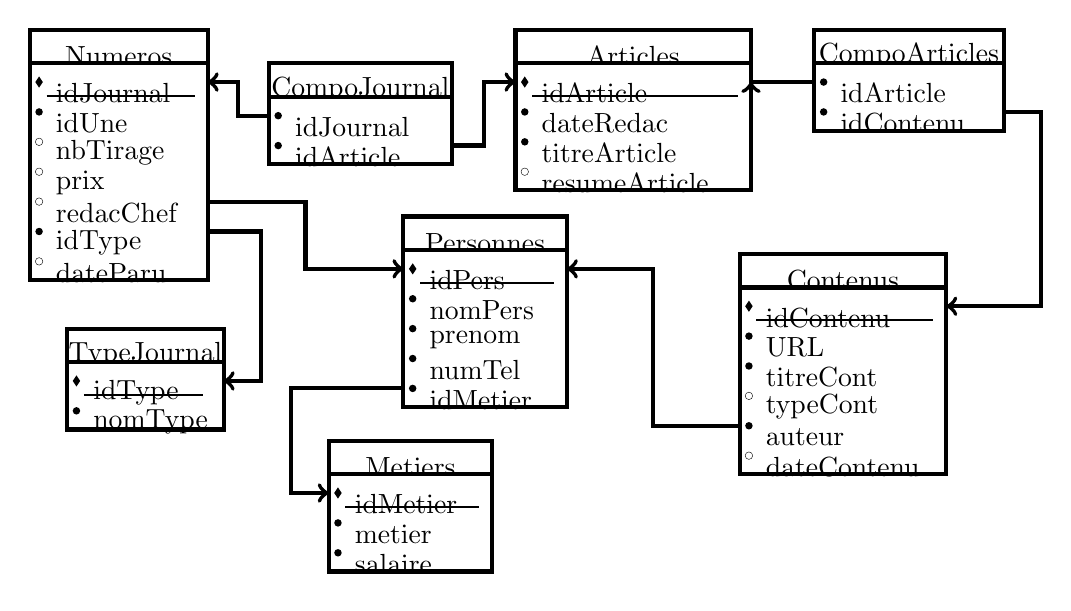
\begin{tikzpicture}[scale=0.9]
\pgftransformxscale{1.000000}
\pgftransformyscale{-1.000000}
\definecolor{dialinecolor}{rgb}{0.000000, 0.000000, 0.000000}
\pgfsetstrokecolor{dialinecolor}
\definecolor{dialinecolor}{rgb}{1.000000, 1.000000, 1.000000}
\pgfsetfillcolor{dialinecolor}
\pgfsetlinewidth{0.100000\du}
\pgfsetdash{}{0pt}
\definecolor{dialinecolor}{rgb}{1.000000, 1.000000, 1.000000}
\pgfsetfillcolor{dialinecolor}
\fill (12.000000\du,14.000000\du)--(12.000000\du,14.900000\du)--(16.380000\du,14.900000\du)--(16.380000\du,14.000000\du)--cycle;
\definecolor{dialinecolor}{rgb}{0.000000, 0.000000, 0.000000}
\pgfsetstrokecolor{dialinecolor}
\draw (12.000000\du,14.000000\du)--(12.000000\du,14.900000\du)--(16.380000\du,14.900000\du)--(16.380000\du,14.000000\du)--cycle;
% setfont left to latex
\definecolor{dialinecolor}{rgb}{0.000000, 0.000000, 0.000000}
\pgfsetstrokecolor{dialinecolor}
\node at (14.190000\du,14.700000\du){Metiers};
\definecolor{dialinecolor}{rgb}{1.000000, 1.000000, 1.000000}
\pgfsetfillcolor{dialinecolor}
\fill (12.000000\du,14.900000\du)--(12.000000\du,17.500000\du)--(16.380000\du,17.500000\du)--(16.380000\du,14.900000\du)--cycle;
\definecolor{dialinecolor}{rgb}{0.000000, 0.000000, 0.000000}
\pgfsetstrokecolor{dialinecolor}
\draw (12.000000\du,14.900000\du)--(12.000000\du,17.500000\du)--(16.380000\du,17.500000\du)--(16.380000\du,14.900000\du)--cycle;
% setfont left to latex
\pgfsetlinewidth{0.010000\du}
\pgfsetmiterjoin
\definecolor{dialinecolor}{rgb}{0.000000, 0.000000, 0.000000}
\pgfsetfillcolor{dialinecolor}
\fill (12.150000\du,15.400000\du)--(12.250000\du,15.550000\du)--(12.350000\du,15.400000\du)--(12.250000\du,15.250000\du)--cycle;
\definecolor{dialinecolor}{rgb}{0.000000, 0.000000, 0.000000}
\pgfsetstrokecolor{dialinecolor}
\node[anchor=west] at (12.450000\du,15.700000\du){idMetier};
\pgfsetlinewidth{0.050000\du}
\definecolor{dialinecolor}{rgb}{0.000000, 0.000000, 0.000000}
\pgfsetstrokecolor{dialinecolor}
\draw (12.450000\du,15.780000\du)--(16.030000\du,15.780000\du);
% setfont left to latex
\pgfsetlinewidth{0.010000\du}
\definecolor{dialinecolor}{rgb}{0.000000, 0.000000, 0.000000}
\pgfsetfillcolor{dialinecolor}
\pgfpathellipse{\pgfpoint{12.250000\du}{16.200000\du}}{\pgfpoint{0.100000\du}{0\du}}{\pgfpoint{0\du}{0.100000\du}}
\pgfusepath{fill}
\definecolor{dialinecolor}{rgb}{0.000000, 0.000000, 0.000000}
\pgfsetstrokecolor{dialinecolor}
\node[anchor=west] at (12.450000\du,16.500000\du){metier};
% setfont left to latex
\pgfsetlinewidth{0.010000\du}
\definecolor{dialinecolor}{rgb}{0.000000, 0.000000, 0.000000}
\pgfsetfillcolor{dialinecolor}
\pgfpathellipse{\pgfpoint{12.250000\du}{17.000000\du}}{\pgfpoint{0.100000\du}{0\du}}{\pgfpoint{0\du}{0.100000\du}}
\pgfusepath{fill}
\definecolor{dialinecolor}{rgb}{0.000000, 0.000000, 0.000000}
\pgfsetstrokecolor{dialinecolor}
\node[anchor=west] at (12.450000\du,17.300000\du){salaire};
\pgfsetlinewidth{0.100000\du}
\pgfsetdash{}{0pt}
\definecolor{dialinecolor}{rgb}{1.000000, 1.000000, 1.000000}
\pgfsetfillcolor{dialinecolor}
\fill (5.000000\du,11.000000\du)--(5.000000\du,11.900000\du)--(9.192500\du,11.900000\du)--(9.192500\du,11.000000\du)--cycle;
\definecolor{dialinecolor}{rgb}{0.000000, 0.000000, 0.000000}
\pgfsetstrokecolor{dialinecolor}
\draw (5.000000\du,11.000000\du)--(5.000000\du,11.900000\du)--(9.192500\du,11.900000\du)--(9.192500\du,11.000000\du)--cycle;
% setfont left to latex
\definecolor{dialinecolor}{rgb}{0.000000, 0.000000, 0.000000}
\pgfsetstrokecolor{dialinecolor}
\node at (7.096250\du,11.700000\du){TypeJournal};
\definecolor{dialinecolor}{rgb}{1.000000, 1.000000, 1.000000}
\pgfsetfillcolor{dialinecolor}
\fill (5.000000\du,11.900000\du)--(5.000000\du,13.700000\du)--(9.192500\du,13.700000\du)--(9.192500\du,11.900000\du)--cycle;
\definecolor{dialinecolor}{rgb}{0.000000, 0.000000, 0.000000}
\pgfsetstrokecolor{dialinecolor}
\draw (5.000000\du,11.900000\du)--(5.000000\du,13.700000\du)--(9.192500\du,13.700000\du)--(9.192500\du,11.900000\du)--cycle;
% setfont left to latex
\pgfsetlinewidth{0.010000\du}
\pgfsetmiterjoin
\definecolor{dialinecolor}{rgb}{0.000000, 0.000000, 0.000000}
\pgfsetfillcolor{dialinecolor}
\fill (5.150000\du,12.400000\du)--(5.250000\du,12.550000\du)--(5.350000\du,12.400000\du)--(5.250000\du,12.250000\du)--cycle;
\definecolor{dialinecolor}{rgb}{0.000000, 0.000000, 0.000000}
\pgfsetstrokecolor{dialinecolor}
\node[anchor=west] at (5.450000\du,12.700000\du){idType};
\pgfsetlinewidth{0.050000\du}
\definecolor{dialinecolor}{rgb}{0.000000, 0.000000, 0.000000}
\pgfsetstrokecolor{dialinecolor}
\draw (5.450000\du,12.780000\du)--(8.645000\du,12.780000\du);
% setfont left to latex
\pgfsetlinewidth{0.010000\du}
\definecolor{dialinecolor}{rgb}{0.000000, 0.000000, 0.000000}
\pgfsetfillcolor{dialinecolor}
\pgfpathellipse{\pgfpoint{5.250000\du}{13.200000\du}}{\pgfpoint{0.100000\du}{0\du}}{\pgfpoint{0\du}{0.100000\du}}
\pgfusepath{fill}
\definecolor{dialinecolor}{rgb}{0.000000, 0.000000, 0.000000}
\pgfsetstrokecolor{dialinecolor}
\node[anchor=west] at (5.450000\du,13.500000\du){nomType};
\pgfsetlinewidth{0.100000\du}
\pgfsetdash{}{0pt}
\definecolor{dialinecolor}{rgb}{1.000000, 1.000000, 1.000000}
\pgfsetfillcolor{dialinecolor}
\fill (14.000000\du,8.000000\du)--(14.000000\du,8.900000\du)--(18.380000\du,8.900000\du)--(18.380000\du,8.000000\du)--cycle;
\definecolor{dialinecolor}{rgb}{0.000000, 0.000000, 0.000000}
\pgfsetstrokecolor{dialinecolor}
\draw (14.000000\du,8.000000\du)--(14.000000\du,8.900000\du)--(18.380000\du,8.900000\du)--(18.380000\du,8.000000\du)--cycle;
% setfont left to latex
\definecolor{dialinecolor}{rgb}{0.000000, 0.000000, 0.000000}
\pgfsetstrokecolor{dialinecolor}
\node at (16.190000\du,8.700000\du){Personnes};
\definecolor{dialinecolor}{rgb}{1.000000, 1.000000, 1.000000}
\pgfsetfillcolor{dialinecolor}
\fill (14.000000\du,8.900000\du)--(14.000000\du,13.100000\du)--(18.380000\du,13.100000\du)--(18.380000\du,8.900000\du)--cycle;
\definecolor{dialinecolor}{rgb}{0.000000, 0.000000, 0.000000}
\pgfsetstrokecolor{dialinecolor}
\draw (14.000000\du,8.900000\du)--(14.000000\du,13.100000\du)--(18.380000\du,13.100000\du)--(18.380000\du,8.900000\du)--cycle;
% setfont left to latex
\pgfsetlinewidth{0.010000\du}
\pgfsetmiterjoin
\definecolor{dialinecolor}{rgb}{0.000000, 0.000000, 0.000000}
\pgfsetfillcolor{dialinecolor}
\fill (14.150000\du,9.400000\du)--(14.250000\du,9.550000\du)--(14.350000\du,9.400000\du)--(14.250000\du,9.250000\du)--cycle;
\definecolor{dialinecolor}{rgb}{0.000000, 0.000000, 0.000000}
\pgfsetstrokecolor{dialinecolor}
\node[anchor=west] at (14.450000\du,9.700000\du){idPers};
\pgfsetlinewidth{0.050000\du}
\definecolor{dialinecolor}{rgb}{0.000000, 0.000000, 0.000000}
\pgfsetstrokecolor{dialinecolor}
\draw (14.450000\du,9.780000\du)--(18.030000\du,9.780000\du);
% setfont left to latex
\pgfsetlinewidth{0.010000\du}
\definecolor{dialinecolor}{rgb}{0.000000, 0.000000, 0.000000}
\pgfsetfillcolor{dialinecolor}
\pgfpathellipse{\pgfpoint{14.250000\du}{10.200000\du}}{\pgfpoint{0.100000\du}{0\du}}{\pgfpoint{0\du}{0.100000\du}}
\pgfusepath{fill}
\definecolor{dialinecolor}{rgb}{0.000000, 0.000000, 0.000000}
\pgfsetstrokecolor{dialinecolor}
\node[anchor=west] at (14.450000\du,10.500000\du){nomPers};
% setfont left to latex
\pgfsetlinewidth{0.010000\du}
\definecolor{dialinecolor}{rgb}{0.000000, 0.000000, 0.000000}
\pgfsetfillcolor{dialinecolor}
\pgfpathellipse{\pgfpoint{14.250000\du}{11.000000\du}}{\pgfpoint{0.100000\du}{0\du}}{\pgfpoint{0\du}{0.100000\du}}
\pgfusepath{fill}
\definecolor{dialinecolor}{rgb}{0.000000, 0.000000, 0.000000}
\pgfsetstrokecolor{dialinecolor}
\node[anchor=west] at (14.450000\du,11.300000\du){prenom};
% setfont left to latex
\pgfsetlinewidth{0.010000\du}
\definecolor{dialinecolor}{rgb}{0.000000, 0.000000, 0.000000}
\pgfsetfillcolor{dialinecolor}
\pgfpathellipse{\pgfpoint{14.250000\du}{11.800000\du}}{\pgfpoint{0.100000\du}{0\du}}{\pgfpoint{0\du}{0.100000\du}}
\pgfusepath{fill}
\definecolor{dialinecolor}{rgb}{0.000000, 0.000000, 0.000000}
\pgfsetstrokecolor{dialinecolor}
\node[anchor=west] at (14.450000\du,12.100000\du){numTel};
% setfont left to latex
\pgfsetlinewidth{0.010000\du}
\definecolor{dialinecolor}{rgb}{0.000000, 0.000000, 0.000000}
\pgfsetfillcolor{dialinecolor}
\pgfpathellipse{\pgfpoint{14.250000\du}{12.600000\du}}{\pgfpoint{0.100000\du}{0\du}}{\pgfpoint{0\du}{0.100000\du}}
\pgfusepath{fill}
\definecolor{dialinecolor}{rgb}{0.000000, 0.000000, 0.000000}
\pgfsetstrokecolor{dialinecolor}
\node[anchor=west] at (14.450000\du,12.900000\du){idMetier};
\pgfsetlinewidth{0.100000\du}
\pgfsetdash{}{0pt}
\definecolor{dialinecolor}{rgb}{1.000000, 1.000000, 1.000000}
\pgfsetfillcolor{dialinecolor}
\fill (17.000000\du,3.000000\du)--(17.000000\du,3.900000\du)--(23.305000\du,3.900000\du)--(23.305000\du,3.000000\du)--cycle;
\definecolor{dialinecolor}{rgb}{0.000000, 0.000000, 0.000000}
\pgfsetstrokecolor{dialinecolor}
\draw (17.000000\du,3.000000\du)--(17.000000\du,3.900000\du)--(23.305000\du,3.900000\du)--(23.305000\du,3.000000\du)--cycle;
% setfont left to latex
\definecolor{dialinecolor}{rgb}{0.000000, 0.000000, 0.000000}
\pgfsetstrokecolor{dialinecolor}
\node at (20.152500\du,3.700000\du){Articles};
\definecolor{dialinecolor}{rgb}{1.000000, 1.000000, 1.000000}
\pgfsetfillcolor{dialinecolor}
\fill (17.000000\du,3.900000\du)--(17.000000\du,7.300000\du)--(23.305000\du,7.300000\du)--(23.305000\du,3.900000\du)--cycle;
\definecolor{dialinecolor}{rgb}{0.000000, 0.000000, 0.000000}
\pgfsetstrokecolor{dialinecolor}
\draw (17.000000\du,3.900000\du)--(17.000000\du,7.300000\du)--(23.305000\du,7.300000\du)--(23.305000\du,3.900000\du)--cycle;
% setfont left to latex
\pgfsetlinewidth{0.010000\du}
\pgfsetmiterjoin
\definecolor{dialinecolor}{rgb}{0.000000, 0.000000, 0.000000}
\pgfsetfillcolor{dialinecolor}
\fill (17.150000\du,4.400000\du)--(17.250000\du,4.550000\du)--(17.350000\du,4.400000\du)--(17.250000\du,4.250000\du)--cycle;
\definecolor{dialinecolor}{rgb}{0.000000, 0.000000, 0.000000}
\pgfsetstrokecolor{dialinecolor}
\node[anchor=west] at (17.450000\du,4.700000\du){idArticle};
\pgfsetlinewidth{0.050000\du}
\definecolor{dialinecolor}{rgb}{0.000000, 0.000000, 0.000000}
\pgfsetstrokecolor{dialinecolor}
\draw (17.450000\du,4.780000\du)--(22.955000\du,4.780000\du);
% setfont left to latex
\pgfsetlinewidth{0.010000\du}
\definecolor{dialinecolor}{rgb}{0.000000, 0.000000, 0.000000}
\pgfsetfillcolor{dialinecolor}
\pgfpathellipse{\pgfpoint{17.250000\du}{5.200000\du}}{\pgfpoint{0.100000\du}{0\du}}{\pgfpoint{0\du}{0.100000\du}}
\pgfusepath{fill}
\definecolor{dialinecolor}{rgb}{0.000000, 0.000000, 0.000000}
\pgfsetstrokecolor{dialinecolor}
\node[anchor=west] at (17.450000\du,5.500000\du){dateRedac};
% setfont left to latex
\pgfsetlinewidth{0.010000\du}
\definecolor{dialinecolor}{rgb}{0.000000, 0.000000, 0.000000}
\pgfsetfillcolor{dialinecolor}
\pgfpathellipse{\pgfpoint{17.250000\du}{6.000000\du}}{\pgfpoint{0.100000\du}{0\du}}{\pgfpoint{0\du}{0.100000\du}}
\pgfusepath{fill}
\definecolor{dialinecolor}{rgb}{0.000000, 0.000000, 0.000000}
\pgfsetstrokecolor{dialinecolor}
\node[anchor=west] at (17.450000\du,6.300000\du){titreArticle};
% setfont left to latex
\pgfsetlinewidth{0.010000\du}
\definecolor{dialinecolor}{rgb}{0.000000, 0.000000, 0.000000}
\pgfsetstrokecolor{dialinecolor}
\pgfpathellipse{\pgfpoint{17.250000\du}{6.800000\du}}{\pgfpoint{0.100000\du}{0\du}}{\pgfpoint{0\du}{0.100000\du}}
\pgfusepath{stroke}
\definecolor{dialinecolor}{rgb}{0.000000, 0.000000, 0.000000}
\pgfsetstrokecolor{dialinecolor}
\node[anchor=west] at (17.450000\du,7.100000\du){resumeArticle};
\pgfsetlinewidth{0.100000\du}
\pgfsetdash{}{0pt}
\definecolor{dialinecolor}{rgb}{1.000000, 1.000000, 1.000000}
\pgfsetfillcolor{dialinecolor}
\fill (23.000000\du,9.000000\du)--(23.000000\du,9.900000\du)--(28.535000\du,9.900000\du)--(28.535000\du,9.000000\du)--cycle;
\definecolor{dialinecolor}{rgb}{0.000000, 0.000000, 0.000000}
\pgfsetstrokecolor{dialinecolor}
\draw (23.000000\du,9.000000\du)--(23.000000\du,9.900000\du)--(28.535000\du,9.900000\du)--(28.535000\du,9.000000\du)--cycle;
% setfont left to latex
\definecolor{dialinecolor}{rgb}{0.000000, 0.000000, 0.000000}
\pgfsetstrokecolor{dialinecolor}
\node at (25.767500\du,9.700000\du){Contenus};
\definecolor{dialinecolor}{rgb}{1.000000, 1.000000, 1.000000}
\pgfsetfillcolor{dialinecolor}
\fill (23.000000\du,9.900000\du)--(23.000000\du,14.900000\du)--(28.535000\du,14.900000\du)--(28.535000\du,9.900000\du)--cycle;
\definecolor{dialinecolor}{rgb}{0.000000, 0.000000, 0.000000}
\pgfsetstrokecolor{dialinecolor}
\draw (23.000000\du,9.900000\du)--(23.000000\du,14.900000\du)--(28.535000\du,14.900000\du)--(28.535000\du,9.900000\du)--cycle;
% setfont left to latex
\pgfsetlinewidth{0.010000\du}
\pgfsetmiterjoin
\definecolor{dialinecolor}{rgb}{0.000000, 0.000000, 0.000000}
\pgfsetfillcolor{dialinecolor}
\fill (23.150000\du,10.400000\du)--(23.250000\du,10.550000\du)--(23.350000\du,10.400000\du)--(23.250000\du,10.250000\du)--cycle;
\definecolor{dialinecolor}{rgb}{0.000000, 0.000000, 0.000000}
\pgfsetstrokecolor{dialinecolor}
\node[anchor=west] at (23.450000\du,10.700000\du){idContenu};
\pgfsetlinewidth{0.050000\du}
\definecolor{dialinecolor}{rgb}{0.000000, 0.000000, 0.000000}
\pgfsetstrokecolor{dialinecolor}
\draw (23.450000\du,10.780000\du)--(28.185000\du,10.780000\du);
% setfont left to latex
\pgfsetlinewidth{0.010000\du}
\definecolor{dialinecolor}{rgb}{0.000000, 0.000000, 0.000000}
\pgfsetfillcolor{dialinecolor}
\pgfpathellipse{\pgfpoint{23.250000\du}{11.200000\du}}{\pgfpoint{0.100000\du}{0\du}}{\pgfpoint{0\du}{0.100000\du}}
\pgfusepath{fill}
\definecolor{dialinecolor}{rgb}{0.000000, 0.000000, 0.000000}
\pgfsetstrokecolor{dialinecolor}
\node[anchor=west] at (23.450000\du,11.500000\du){URL};
% setfont left to latex
\pgfsetlinewidth{0.010000\du}
\definecolor{dialinecolor}{rgb}{0.000000, 0.000000, 0.000000}
\pgfsetfillcolor{dialinecolor}
\pgfpathellipse{\pgfpoint{23.250000\du}{12.000000\du}}{\pgfpoint{0.100000\du}{0\du}}{\pgfpoint{0\du}{0.100000\du}}
\pgfusepath{fill}
\definecolor{dialinecolor}{rgb}{0.000000, 0.000000, 0.000000}
\pgfsetstrokecolor{dialinecolor}
\node[anchor=west] at (23.450000\du,12.300000\du){titreCont};
% setfont left to latex
\pgfsetlinewidth{0.010000\du}
\definecolor{dialinecolor}{rgb}{0.000000, 0.000000, 0.000000}
\pgfsetstrokecolor{dialinecolor}
\pgfpathellipse{\pgfpoint{23.250000\du}{12.800000\du}}{\pgfpoint{0.100000\du}{0\du}}{\pgfpoint{0\du}{0.100000\du}}
\pgfusepath{stroke}
\definecolor{dialinecolor}{rgb}{0.000000, 0.000000, 0.000000}
\pgfsetstrokecolor{dialinecolor}
\node[anchor=west] at (23.450000\du,13.100000\du){typeCont};
% setfont left to latex
\pgfsetlinewidth{0.010000\du}
\definecolor{dialinecolor}{rgb}{0.000000, 0.000000, 0.000000}
\pgfsetfillcolor{dialinecolor}
\pgfpathellipse{\pgfpoint{23.250000\du}{13.600000\du}}{\pgfpoint{0.100000\du}{0\du}}{\pgfpoint{0\du}{0.100000\du}}
\pgfusepath{fill}
\definecolor{dialinecolor}{rgb}{0.000000, 0.000000, 0.000000}
\pgfsetstrokecolor{dialinecolor}
\node[anchor=west] at (23.450000\du,13.900000\du){auteur};
% setfont left to latex
\pgfsetlinewidth{0.010000\du}
\definecolor{dialinecolor}{rgb}{0.000000, 0.000000, 0.000000}
\pgfsetstrokecolor{dialinecolor}
\pgfpathellipse{\pgfpoint{23.250000\du}{14.400000\du}}{\pgfpoint{0.100000\du}{0\du}}{\pgfpoint{0\du}{0.100000\du}}
\pgfusepath{stroke}
\definecolor{dialinecolor}{rgb}{0.000000, 0.000000, 0.000000}
\pgfsetstrokecolor{dialinecolor}
\node[anchor=west] at (23.450000\du,14.700000\du){dateContenu};
\pgfsetlinewidth{0.100000\du}
\pgfsetdash{}{0pt}
\definecolor{dialinecolor}{rgb}{1.000000, 1.000000, 1.000000}
\pgfsetfillcolor{dialinecolor}
\fill (4.000000\du,3.000000\du)--(4.000000\du,3.900000\du)--(8.765000\du,3.900000\du)--(8.765000\du,3.000000\du)--cycle;
\definecolor{dialinecolor}{rgb}{0.000000, 0.000000, 0.000000}
\pgfsetstrokecolor{dialinecolor}
\draw (4.000000\du,3.000000\du)--(4.000000\du,3.900000\du)--(8.765000\du,3.900000\du)--(8.765000\du,3.000000\du)--cycle;
% setfont left to latex
\definecolor{dialinecolor}{rgb}{0.000000, 0.000000, 0.000000}
\pgfsetstrokecolor{dialinecolor}
\node at (6.382500\du,3.700000\du){Numeros};
\definecolor{dialinecolor}{rgb}{1.000000, 1.000000, 1.000000}
\pgfsetfillcolor{dialinecolor}
\fill (4.000000\du,3.900000\du)--(4.000000\du,9.700000\du)--(8.765000\du,9.700000\du)--(8.765000\du,3.900000\du)--cycle;
\definecolor{dialinecolor}{rgb}{0.000000, 0.000000, 0.000000}
\pgfsetstrokecolor{dialinecolor}
\draw (4.000000\du,3.900000\du)--(4.000000\du,9.700000\du)--(8.765000\du,9.700000\du)--(8.765000\du,3.900000\du)--cycle;
% setfont left to latex
\pgfsetlinewidth{0.010000\du}
\pgfsetmiterjoin
\definecolor{dialinecolor}{rgb}{0.000000, 0.000000, 0.000000}
\pgfsetfillcolor{dialinecolor}
\fill (4.150000\du,4.400000\du)--(4.250000\du,4.550000\du)--(4.350000\du,4.400000\du)--(4.250000\du,4.250000\du)--cycle;
\definecolor{dialinecolor}{rgb}{0.000000, 0.000000, 0.000000}
\pgfsetstrokecolor{dialinecolor}
\node[anchor=west] at (4.450000\du,4.700000\du){idJournal};
\pgfsetlinewidth{0.050000\du}
\definecolor{dialinecolor}{rgb}{0.000000, 0.000000, 0.000000}
\pgfsetstrokecolor{dialinecolor}
\draw (4.450000\du,4.780000\du)--(8.415000\du,4.780000\du);
% setfont left to latex
\pgfsetlinewidth{0.010000\du}
\definecolor{dialinecolor}{rgb}{0.000000, 0.000000, 0.000000}
\pgfsetfillcolor{dialinecolor}
\pgfpathellipse{\pgfpoint{4.250000\du}{5.200000\du}}{\pgfpoint{0.100000\du}{0\du}}{\pgfpoint{0\du}{0.100000\du}}
\pgfusepath{fill}
\definecolor{dialinecolor}{rgb}{0.000000, 0.000000, 0.000000}
\pgfsetstrokecolor{dialinecolor}
\node[anchor=west] at (4.450000\du,5.500000\du){idUne};
% setfont left to latex
\pgfsetlinewidth{0.010000\du}
\definecolor{dialinecolor}{rgb}{0.000000, 0.000000, 0.000000}
\pgfsetstrokecolor{dialinecolor}
\pgfpathellipse{\pgfpoint{4.250000\du}{6.000000\du}}{\pgfpoint{0.100000\du}{0\du}}{\pgfpoint{0\du}{0.100000\du}}
\pgfusepath{stroke}
\definecolor{dialinecolor}{rgb}{0.000000, 0.000000, 0.000000}
\pgfsetstrokecolor{dialinecolor}
\node[anchor=west] at (4.450000\du,6.300000\du){nbTirage};
% setfont left to latex
\pgfsetlinewidth{0.010000\du}
\definecolor{dialinecolor}{rgb}{0.000000, 0.000000, 0.000000}
\pgfsetstrokecolor{dialinecolor}
\pgfpathellipse{\pgfpoint{4.250000\du}{6.800000\du}}{\pgfpoint{0.100000\du}{0\du}}{\pgfpoint{0\du}{0.100000\du}}
\pgfusepath{stroke}
\definecolor{dialinecolor}{rgb}{0.000000, 0.000000, 0.000000}
\pgfsetstrokecolor{dialinecolor}
\node[anchor=west] at (4.450000\du,7.100000\du){prix};
% setfont left to latex
\pgfsetlinewidth{0.010000\du}
\definecolor{dialinecolor}{rgb}{0.000000, 0.000000, 0.000000}
\pgfsetstrokecolor{dialinecolor}
\pgfpathellipse{\pgfpoint{4.250000\du}{7.600000\du}}{\pgfpoint{0.100000\du}{0\du}}{\pgfpoint{0\du}{0.100000\du}}
\pgfusepath{stroke}
\definecolor{dialinecolor}{rgb}{0.000000, 0.000000, 0.000000}
\pgfsetstrokecolor{dialinecolor}
\node[anchor=west] at (4.450000\du,7.900000\du){redacChef};
% setfont left to latex
\pgfsetlinewidth{0.010000\du}
\definecolor{dialinecolor}{rgb}{0.000000, 0.000000, 0.000000}
\pgfsetfillcolor{dialinecolor}
\pgfpathellipse{\pgfpoint{4.250000\du}{8.400000\du}}{\pgfpoint{0.100000\du}{0\du}}{\pgfpoint{0\du}{0.100000\du}}
\pgfusepath{fill}
\definecolor{dialinecolor}{rgb}{0.000000, 0.000000, 0.000000}
\pgfsetstrokecolor{dialinecolor}
\node[anchor=west] at (4.450000\du,8.700000\du){idType};
% setfont left to latex
\pgfsetlinewidth{0.010000\du}
\definecolor{dialinecolor}{rgb}{0.000000, 0.000000, 0.000000}
\pgfsetstrokecolor{dialinecolor}
\pgfpathellipse{\pgfpoint{4.250000\du}{9.200000\du}}{\pgfpoint{0.100000\du}{0\du}}{\pgfpoint{0\du}{0.100000\du}}
\pgfusepath{stroke}
\definecolor{dialinecolor}{rgb}{0.000000, 0.000000, 0.000000}
\pgfsetstrokecolor{dialinecolor}
\node[anchor=west] at (4.450000\du,9.500000\du){dateParu};
\pgfsetlinewidth{0.100000\du}
\pgfsetdash{}{0pt}
\definecolor{dialinecolor}{rgb}{1.000000, 1.000000, 1.000000}
\pgfsetfillcolor{dialinecolor}
\fill (25.000000\du,3.000000\du)--(25.000000\du,3.900000\du)--(30.067500\du,3.900000\du)--(30.067500\du,3.000000\du)--cycle;
\definecolor{dialinecolor}{rgb}{0.000000, 0.000000, 0.000000}
\pgfsetstrokecolor{dialinecolor}
\draw (25.000000\du,3.000000\du)--(25.000000\du,3.900000\du)--(30.067500\du,3.900000\du)--(30.067500\du,3.000000\du)--cycle;
% setfont left to latex
\definecolor{dialinecolor}{rgb}{0.000000, 0.000000, 0.000000}
\pgfsetstrokecolor{dialinecolor}
\node at (27.533750\du,3.700000\du){CompoArticles};
\definecolor{dialinecolor}{rgb}{1.000000, 1.000000, 1.000000}
\pgfsetfillcolor{dialinecolor}
\fill (25.000000\du,3.900000\du)--(25.000000\du,5.700000\du)--(30.067500\du,5.700000\du)--(30.067500\du,3.900000\du)--cycle;
\definecolor{dialinecolor}{rgb}{0.000000, 0.000000, 0.000000}
\pgfsetstrokecolor{dialinecolor}
\draw (25.000000\du,3.900000\du)--(25.000000\du,5.700000\du)--(30.067500\du,5.700000\du)--(30.067500\du,3.900000\du)--cycle;
% setfont left to latex
\pgfsetlinewidth{0.010000\du}
\definecolor{dialinecolor}{rgb}{0.000000, 0.000000, 0.000000}
\pgfsetfillcolor{dialinecolor}
\pgfpathellipse{\pgfpoint{25.250000\du}{4.400000\du}}{\pgfpoint{0.100000\du}{0\du}}{\pgfpoint{0\du}{0.100000\du}}
\pgfusepath{fill}
\definecolor{dialinecolor}{rgb}{0.000000, 0.000000, 0.000000}
\pgfsetstrokecolor{dialinecolor}
\node[anchor=west] at (25.450000\du,4.700000\du){idArticle};
% setfont left to latex
\pgfsetlinewidth{0.010000\du}
\definecolor{dialinecolor}{rgb}{0.000000, 0.000000, 0.000000}
\pgfsetfillcolor{dialinecolor}
\pgfpathellipse{\pgfpoint{25.250000\du}{5.200000\du}}{\pgfpoint{0.100000\du}{0\du}}{\pgfpoint{0\du}{0.100000\du}}
\pgfusepath{fill}
\definecolor{dialinecolor}{rgb}{0.000000, 0.000000, 0.000000}
\pgfsetstrokecolor{dialinecolor}
\node[anchor=west] at (25.450000\du,5.500000\du){idContenu};
\pgfsetlinewidth{0.100000\du}
\pgfsetdash{}{0pt}
\definecolor{dialinecolor}{rgb}{1.000000, 1.000000, 1.000000}
\pgfsetfillcolor{dialinecolor}
\fill (10.400000\du,3.900000\du)--(10.400000\du,4.800000\du)--(15.295000\du,4.800000\du)--(15.295000\du,3.900000\du)--cycle;
\definecolor{dialinecolor}{rgb}{0.000000, 0.000000, 0.000000}
\pgfsetstrokecolor{dialinecolor}
\draw (10.400000\du,3.900000\du)--(10.400000\du,4.800000\du)--(15.295000\du,4.800000\du)--(15.295000\du,3.900000\du)--cycle;
% setfont left to latex
\definecolor{dialinecolor}{rgb}{0.000000, 0.000000, 0.000000}
\pgfsetstrokecolor{dialinecolor}
\node at (12.847500\du,4.600000\du){CompoJournal};
\definecolor{dialinecolor}{rgb}{1.000000, 1.000000, 1.000000}
\pgfsetfillcolor{dialinecolor}
\fill (10.400000\du,4.800000\du)--(10.400000\du,6.600000\du)--(15.295000\du,6.600000\du)--(15.295000\du,4.800000\du)--cycle;
\definecolor{dialinecolor}{rgb}{0.000000, 0.000000, 0.000000}
\pgfsetstrokecolor{dialinecolor}
\draw (10.400000\du,4.800000\du)--(10.400000\du,6.600000\du)--(15.295000\du,6.600000\du)--(15.295000\du,4.800000\du)--cycle;
% setfont left to latex
\pgfsetlinewidth{0.010000\du}
\definecolor{dialinecolor}{rgb}{0.000000, 0.000000, 0.000000}
\pgfsetfillcolor{dialinecolor}
\pgfpathellipse{\pgfpoint{10.650000\du}{5.300000\du}}{\pgfpoint{0.100000\du}{0\du}}{\pgfpoint{0\du}{0.100000\du}}
\pgfusepath{fill}
\definecolor{dialinecolor}{rgb}{0.000000, 0.000000, 0.000000}
\pgfsetstrokecolor{dialinecolor}
\node[anchor=west] at (10.850000\du,5.600000\du){idJournal};
% setfont left to latex
\pgfsetlinewidth{0.010000\du}
\definecolor{dialinecolor}{rgb}{0.000000, 0.000000, 0.000000}
\pgfsetfillcolor{dialinecolor}
\pgfpathellipse{\pgfpoint{10.650000\du}{6.100000\du}}{\pgfpoint{0.100000\du}{0\du}}{\pgfpoint{0\du}{0.100000\du}}
\pgfusepath{fill}
\definecolor{dialinecolor}{rgb}{0.000000, 0.000000, 0.000000}
\pgfsetstrokecolor{dialinecolor}
\node[anchor=west] at (10.850000\du,6.400000\du){idArticle};
\pgfsetlinewidth{0.100000\du}
\pgfsetdash{}{0pt}
\pgfsetdash{}{0pt}
\pgfsetmiterjoin
\pgfsetbuttcap
{
\definecolor{dialinecolor}{rgb}{0.000000, 0.000000, 0.000000}
\pgfsetfillcolor{dialinecolor}
% was here!!!
\pgfsetarrowsend{to}
{\pgfsetcornersarced{\pgfpoint{0.000000\du}{0.000000\du}}\definecolor{dialinecolor}{rgb}{0.000000, 0.000000, 0.000000}
\pgfsetstrokecolor{dialinecolor}
\draw (10.400000\du,5.300000\du)--(9.582500\du,5.300000\du)--(9.582500\du,4.400000\du)--(8.765000\du,4.400000\du);
}}
% setfont left to latex
\pgfsetlinewidth{0.100000\du}
\pgfsetdash{}{0pt}
\pgfsetdash{}{0pt}
\pgfsetmiterjoin
\pgfsetbuttcap
{
\definecolor{dialinecolor}{rgb}{0.000000, 0.000000, 0.000000}
\pgfsetfillcolor{dialinecolor}
% was here!!!
\pgfsetarrowsend{to}
{\pgfsetcornersarced{\pgfpoint{0.000000\du}{0.000000\du}}\definecolor{dialinecolor}{rgb}{0.000000, 0.000000, 0.000000}
\pgfsetstrokecolor{dialinecolor}
\draw (25.000000\du,4.400000\du)--(25.000000\du,4.400000\du)--(23.305000\du,4.400000\du)--(23.305000\du,4.400000\du);
}}
% setfont left to latex
\pgfsetlinewidth{0.100000\du}
\pgfsetdash{}{0pt}
\pgfsetdash{}{0pt}
\pgfsetmiterjoin
\pgfsetbuttcap
{
\definecolor{dialinecolor}{rgb}{0.000000, 0.000000, 0.000000}
\pgfsetfillcolor{dialinecolor}
% was here!!!
\pgfsetarrowsend{to}
{\pgfsetcornersarced{\pgfpoint{0.000000\du}{0.000000\du}}\definecolor{dialinecolor}{rgb}{0.000000, 0.000000, 0.000000}
\pgfsetstrokecolor{dialinecolor}
\draw (15.295000\du,6.100000\du)--(16.147500\du,6.100000\du)--(16.147500\du,4.400000\du)--(17.000000\du,4.400000\du);
}}
% setfont left to latex
\pgfsetlinewidth{0.100000\du}
\pgfsetdash{}{0pt}
\pgfsetdash{}{0pt}
\pgfsetmiterjoin
\pgfsetbuttcap
{
\definecolor{dialinecolor}{rgb}{0.000000, 0.000000, 0.000000}
\pgfsetfillcolor{dialinecolor}
% was here!!!
\pgfsetarrowsend{to}
{\pgfsetcornersarced{\pgfpoint{0.000000\du}{0.000000\du}}\definecolor{dialinecolor}{rgb}{0.000000, 0.000000, 0.000000}
\pgfsetstrokecolor{dialinecolor}
\draw (30.067500\du,5.200000\du)--(31.067500\du,5.200000\du)--(31.067500\du,10.400000\du)--(28.535000\du,10.400000\du);
}}
% setfont left to latex
\pgfsetlinewidth{0.100000\du}
\pgfsetdash{}{0pt}
\pgfsetdash{}{0pt}
\pgfsetmiterjoin
\pgfsetbuttcap
{
\definecolor{dialinecolor}{rgb}{0.000000, 0.000000, 0.000000}
\pgfsetfillcolor{dialinecolor}
% was here!!!
\pgfsetarrowsend{to}
{\pgfsetcornersarced{\pgfpoint{0.000000\du}{0.000000\du}}\definecolor{dialinecolor}{rgb}{0.000000, 0.000000, 0.000000}
\pgfsetstrokecolor{dialinecolor}
\draw (8.765000\du,7.600000\du)--(11.382500\du,7.600000\du)--(11.382500\du,9.400000\du)--(14.000000\du,9.400000\du);
}}
% setfont left to latex
\pgfsetlinewidth{0.100000\du}
\pgfsetdash{}{0pt}
\pgfsetdash{}{0pt}
\pgfsetmiterjoin
\pgfsetbuttcap
{
\definecolor{dialinecolor}{rgb}{0.000000, 0.000000, 0.000000}
\pgfsetfillcolor{dialinecolor}
% was here!!!
\pgfsetarrowsend{to}
{\pgfsetcornersarced{\pgfpoint{0.000000\du}{0.000000\du}}\definecolor{dialinecolor}{rgb}{0.000000, 0.000000, 0.000000}
\pgfsetstrokecolor{dialinecolor}
\draw (23.000000\du,13.600000\du)--(20.690000\du,13.600000\du)--(20.690000\du,9.400000\du)--(18.380000\du,9.400000\du);
}}
% setfont left to latex
\pgfsetlinewidth{0.100000\du}
\pgfsetdash{}{0pt}
\pgfsetdash{}{0pt}
\pgfsetmiterjoin
\pgfsetbuttcap
{
\definecolor{dialinecolor}{rgb}{0.000000, 0.000000, 0.000000}
\pgfsetfillcolor{dialinecolor}
% was here!!!
\pgfsetarrowsend{to}
{\pgfsetcornersarced{\pgfpoint{0.000000\du}{0.000000\du}}\definecolor{dialinecolor}{rgb}{0.000000, 0.000000, 0.000000}
\pgfsetstrokecolor{dialinecolor}
\draw (8.765000\du,8.400000\du)--(10.192500\du,8.400000\du)--(10.192500\du,12.400000\du)--(9.192500\du,12.400000\du);
}}
% setfont left to latex
\pgfsetlinewidth{0.100000\du}
\pgfsetdash{}{0pt}
\pgfsetdash{}{0pt}
\pgfsetmiterjoin
\pgfsetbuttcap
{
\definecolor{dialinecolor}{rgb}{0.000000, 0.000000, 0.000000}
\pgfsetfillcolor{dialinecolor}
% was here!!!
\pgfsetarrowsend{to}
{\pgfsetcornersarced{\pgfpoint{0.000000\du}{0.000000\du}}\definecolor{dialinecolor}{rgb}{0.000000, 0.000000, 0.000000}
\pgfsetstrokecolor{dialinecolor}
\draw (14.000000\du,12.600000\du)--(11.000000\du,12.600000\du)--(11.000000\du,15.400000\du)--(12.000000\du,15.400000\du);
}}
% setfont left to latex
\end{tikzpicture}
